% Copyright (c) 2024, Francisco Fernandez
% License: CC BY-SA 4.0
%   https://github.com/fernandezfran/thesis/blob/main/LICENSE
\subsection{Formación de clusters}\label{s:clusters}

Analizando la formación de clusters por medio del algoritmo DBSCAN 
\cite{ester1996}, en el cual puede definirse un radio de corte para el cual se 
deja de considerar que los átomos están enlazados entre sí (es decir, formando 
clusters), se encuentra que las estructuras amorfas de silicio no pueden ser 
clasificadas en diferentes tipos de clusters, las mismas reflejan más bien 
una red amorfa. Esto viene de interpretar los gráficos que se presentan en la 
Figura \ref{fig:clusters}. 
\begin{figure}[h!]
    \centering
    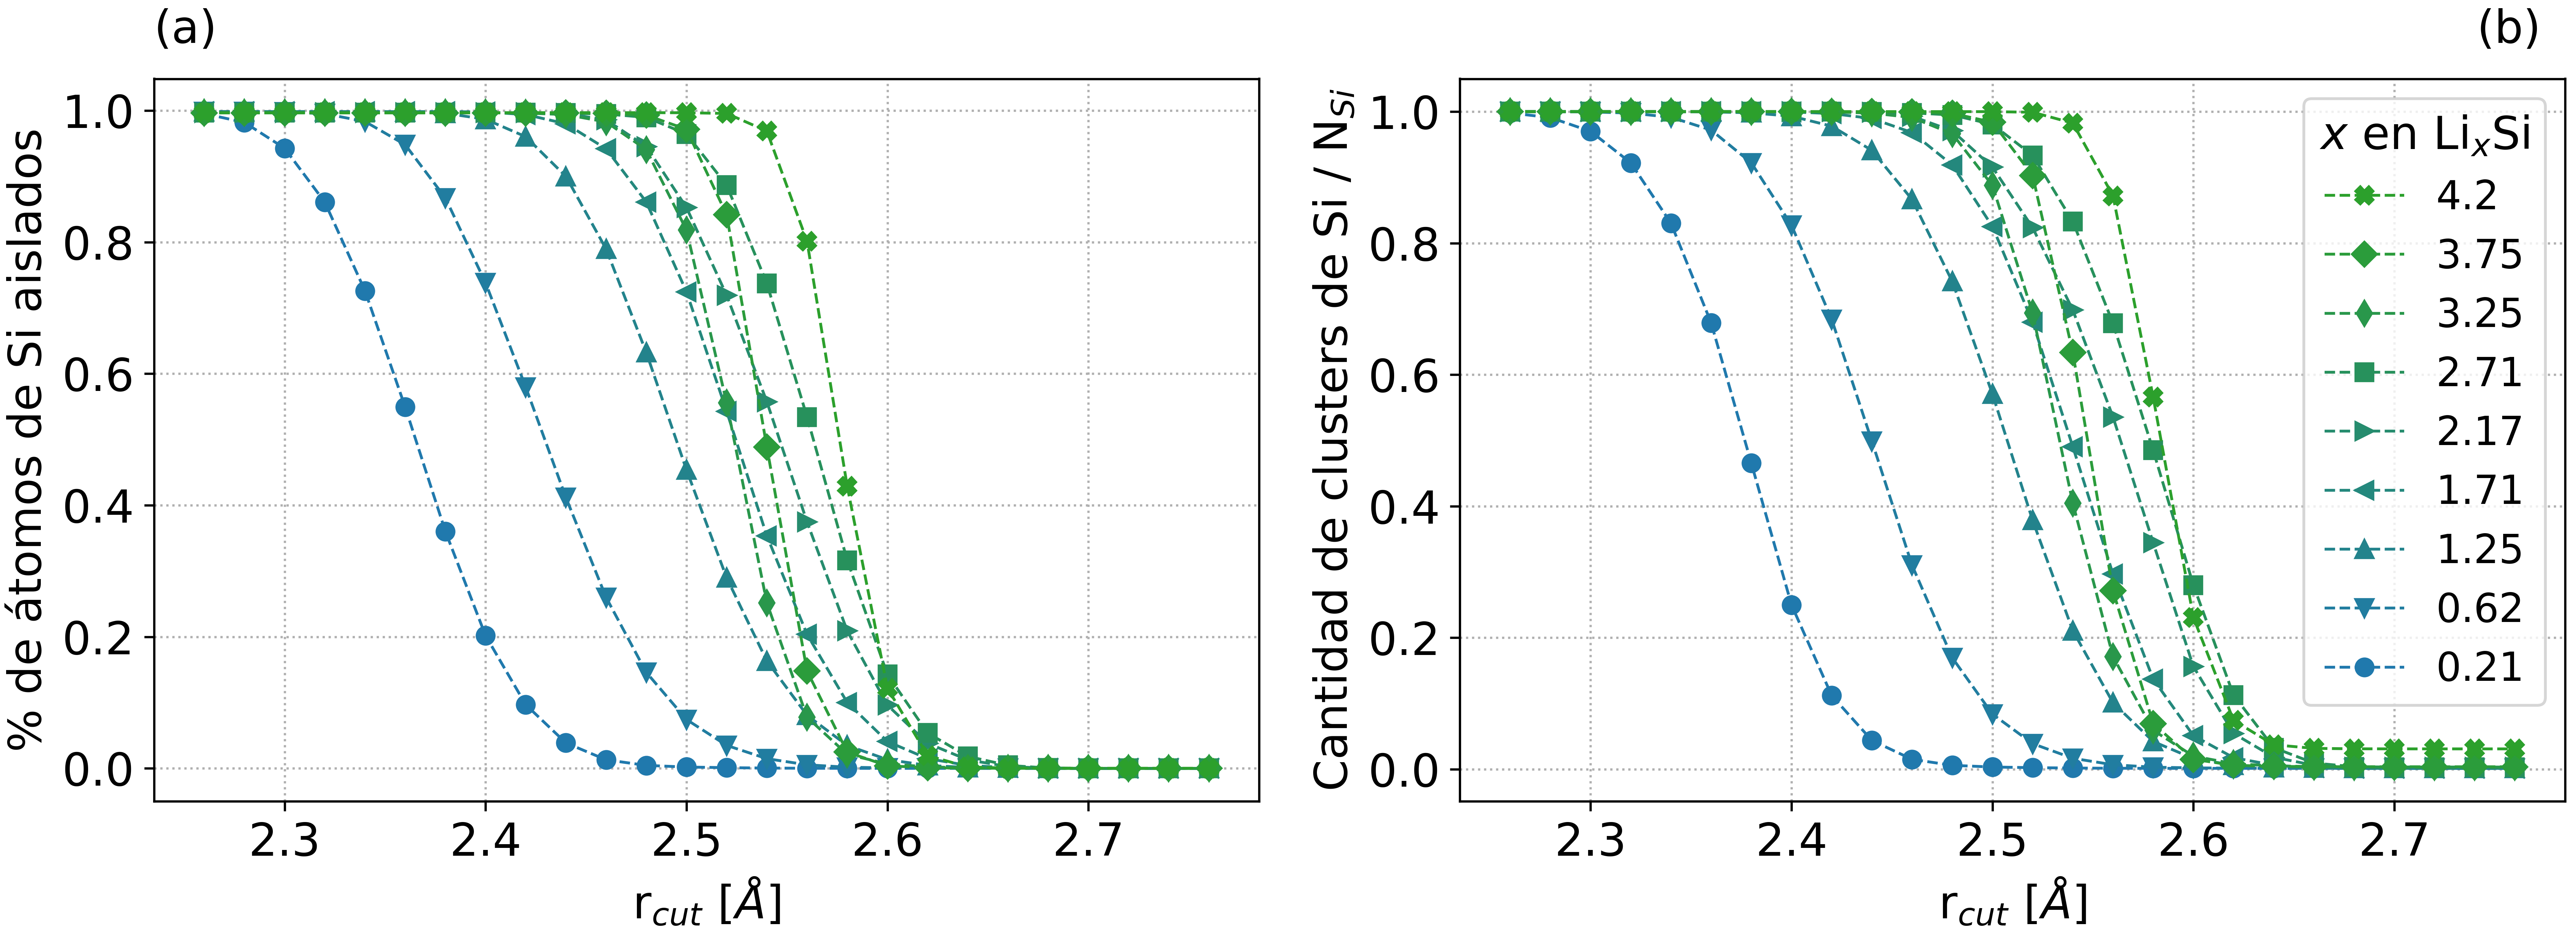
\includegraphics[width=\textwidth]{Silicio/caracterizacion/resultados/clusters/clusters.png}
    \caption{Formación de clusters indicando una red amorfa de silicio. (a) 
    Fracción de átomos de Si aislados en función de la elección del
    radio de corte. (b) Número de clusters de Si sobre el número total de átomos 
    de Si.}
    \label{fig:clusters}
\end{figure}

En particular, en la Figura \ref{fig:clusters}a se define la fracción 
de átomos de Si que están a una distancia mayor que $r_{cut}$ de otros átomos de 
Si. Cuando el radio de corte es mayor que la distancia a la cual termina el 
primer pico de la RDF$_{\text{Si}-\text{Si}}$, no se tienen átomos de Si que cumplan esta 
propiedad, es decir, no hay átomos de Si que se encuentren aislados en el sistema,
incluso a concentraciones altas de Li. Esto refleja que el a-Si se comporta como 
una red en la cual todos los átomos de silicio están interconectados entre sí, 
cosa que también se puede deducir de la Figura \ref{fig:clusters}b, en la cual 
se tiene que cuando el radio de corte es menor que el primer pico de la RDF$_{\text{Si}-\text{Si}}$ 
el número de clusters es igual al número de átomos de Si, pero que cuando este 
radio es más grande que la distancia a la cual termina el primer pico, hay un 
solo cluster.
